\hypertarget{conclusion}{%
\chapter{Conclusion}\label{conclusion}}

\section{Conclusion de l'étude}

Nous avons tout d'abord vu avec notre modèle de simulation qu'il fallait tout d'abord limité l'influence de l'aléatoire de notre simulations

\section{Piste d'amélioration}

\subsection{Changer architecture du réseau (Barabasi)}
Nous avons envisagé de changer la \textbf{topologie} \footnote{Topologie: Tel que la topologie d'un graffe il s'agit de la façon dont sont connecté nos neurones entre eux.}. Pour passer à une topologie dite \textbf{scalefree}. Qui est justement celle utilisé dans l'article d'origine. Cette architecture ressemble à ça:

\begin{figure}[h!]
\begin{center}
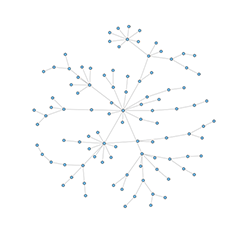
\includegraphics[width=10.5cm,height=10.5cm]{./images/scalefree.png}
\end{center}
\caption{Architecture scale-free}
\label{scale_free}
\end{figure}
\subsection{Réinterprétation de l'expérience}

Nous pouvons interpréter tout le réseau comme un utilisateur et cet entretient comme le temps qu'il accorde à la rumeur.

Cela permettrait
\section{Les apports du stage}
\subsection{les apports au monde}
Grâce à ce stage les chercheurs du laboratoire auront une idée plus précise de la diffusion d'un echo dans un réservoir et comment y créer un entretient ce qui sera utile pour leurs futures expériences. Cela permettra de mieux appréhender certains problèmes.
\subsection{les apports personels}
Comme dit pendant mon introduction, avant ce stage je n'avais aucune connaissance des réseaux de neurones, ce stage m'a donc permis de m'ouvrir a ce nouveau sujet passionnant, et m'a permis d'obtenir des compétence nécéssaire à mon cursus universitaire. Il m'a permis d'affiné mes méthodes de travail grâce à l'apprentissage de l'utilisation de GitHub et Colab. J'ai amélioré ma rédaction grace à l'approfondissement
du LaTeX. Il m'a permis d'affiner mon analyse de par l'analyse de mes résultats.
